\chapter{Graph Theory and Network Science}

This chapter builds the mathematical language we will use throughout the entire workbook. A disease cannot spread without a contact network, and a Graph Neural Network (GNN) cannot operate without a graph. Before we simulate outbreaks, detect sources, or implement any model, we need to speak fluently in the vocabulary of graph theory.

We start from absolute zero. If you have never seen a matrix before, this chapter will bring you to the point where you can compute a normalised Laplacian by hand. If you are already comfortable with linear algebra, use the Building Blocks boxes at the start of each section as quick reference cards and spend your time on the epidemic interpretation paragraphs.

\begin{analogybox}{Why a Disease Needs a Map}
Imagine trying to trace who started a rumour in a school. You need to know who talks to whom --- the \emph{contact structure}. Without a map of friendships, you cannot reason about how the rumour spread. Graph theory is precisely the science of such maps. It gives us a formal language to write down ``who is connected to whom'' in a way that a computer can operate on.
\end{analogybox}

% =============================================================================
\section{Formal Graph Definitions}
\label{sec:graph_definitions}
% =============================================================================

\begin{conceptbox}{Building Blocks for This Section}
Before we define anything, let us introduce the notation we will use:
\begin{itemize}[noitemsep]
    \item $G$ --- a graph (the whole network)
    \item $\mathcal{V}$ --- the set of vertices (nodes, people, locations)
    \item $\mathcal{E}$ --- the set of edges (connections, contacts, links)
    \item $n = |\mathcal{V}|$ --- the number of nodes (the vertical bars $|\cdot|$ mean ``size of the set'')
    \item $m = |\mathcal{E}|$ --- the number of edges
    \item $\subseteq$ --- ``is a subset of'' (every element on the left also belongs to the right)
    \item $\times$ --- the Cartesian product: $\mathcal{V} \times \mathcal{V}$ means all possible ordered pairs of nodes
    \item $\in$ --- ``is an element of'' (e.g.\ $v \in \mathcal{V}$ means ``$v$ is one of the nodes'')
    \item $\iff$ --- ``if and only if'' (both directions hold simultaneously)
\end{itemize}
\end{conceptbox}

\begin{conceptbox}{The Graph $G = (\mathcal{V}, \mathcal{E})$}
A \textbf{graph} $G$ is an ordered pair $G = (\mathcal{V}, \mathcal{E})$, where:
\begin{itemize}[noitemsep]
    \item $\mathcal{V} = \{v_1, v_2, \dots, v_n\}$ is the finite, non-empty set of \textbf{vertices} (also called \textit{nodes}), with $|\mathcal{V}| = n$.
    \item $\mathcal{E} \subseteq \mathcal{V} \times \mathcal{V}$ is the set of \textbf{edges} (also called \textit{links}), with $|\mathcal{E}| = m$.
\end{itemize}
The \textbf{density} of the graph is $\rho = \frac{2m}{n(n-1)}$ for undirected graphs. The number $n(n-1)/2$ is the maximum possible number of edges, so $\rho$ tells you what fraction of all possible connections actually exist.
\end{conceptbox}

\begin{examplebox}{Reading $G = (\mathcal{V}, \mathcal{E})$ Aloud}
``$G = (\mathcal{V}, \mathcal{E})$'' is read as: ``$G$ is a graph with node set $\mathcal{V}$ and edge set $\mathcal{E}$.''

A concrete example: a classroom has 4 students, and students 1--2, 2--3, and 3--4 sit next to each other.
\[
\mathcal{V} = \{1, 2, 3, 4\}, \qquad \mathcal{E} = \{\{1,2\},\, \{2,3\},\, \{3,4\}\}
\]
$n = 4$, $m = 3$, density $= \frac{2 \times 3}{4 \times 3} = \frac{6}{12} = 0.5$.
\end{examplebox}

\begin{keyinsight}{Why This Matters for Epidemics}
Every epidemic model requires a contact network. Each person is a node. Each contact (a handshake, a shared meal, a conversation) is an edge. A graph $G = (\mathcal{V}, \mathcal{E})$ is the minimal formal structure needed to describe who can potentially infect whom.
\end{keyinsight}

\subsection{Undirected and Directed Graphs}

\begin{conceptbox}{Directed vs.\ Undirected}
\begin{itemize}[noitemsep]
    \item \textbf{Undirected graph:} The edge relation is symmetric: $(u,v) \in \mathcal{E} \iff (v,u) \in \mathcal{E}$. We represent an undirected edge as the unordered pair $\{u,v\}$. The \textbf{degree} of node $v$ is $k_v = |\mathcal{N}(v)|$, the number of its neighbours. The \textbf{neighbourhood} is $\mathcal{N}(v) = \{u \in \mathcal{V} \mid \{u,v\} \in \mathcal{E}\}$.
    \item \textbf{Directed graph (digraph):} Edges are ordered pairs $(u \to v)$. Each node has an \textbf{in-degree} $k_v^{\mathrm{in}} = |\{u \mid (u,v) \in \mathcal{E}\}|$ (arrows pointing \emph{in}) and an \textbf{out-degree} $k_v^{\mathrm{out}} = |\{w \mid (v,w) \in \mathcal{E}\}|$ (arrows pointing \emph{out}).
\end{itemize}
In epidemic contact networks we typically use undirected edges: if Alice can infect Bob, Bob can also infect Alice.
\end{conceptbox}

\begin{examplebox}{Degree by Hand}
Classroom graph $\mathcal{E} = \{\{1,2\}, \{2,3\}, \{3,4\}\}$:
\begin{itemize}[noitemsep]
    \item $\mathcal{N}(1) = \{2\}$, so $k_1 = 1$.
    \item $\mathcal{N}(2) = \{1, 3\}$, so $k_2 = 2$.
    \item $\mathcal{N}(3) = \{2, 4\}$, so $k_3 = 2$.
    \item $\mathcal{N}(4) = \{3\}$, so $k_4 = 1$.
\end{itemize}
The sum of all degrees: $1+2+2+1=6 = 2 \times 3 = 2m$. This is always true: every edge contributes exactly 2 to the total degree sum (once per endpoint). This is called the \textbf{handshaking lemma}.
\end{examplebox}

\begin{center}
\begin{tikzpicture}[
  node/.style={circle, draw=blue!60!black, fill=blue!8, thick, minimum size=9mm, font=\small\bfseries},
  >=Stealth, thick
]
\node[font=\bfseries\sffamily] at (1.5, 2.4) {Undirected};
\node[node] (u1) at (0,1)   {1};
\node[node] (u2) at (1.5,1.8) {2};
\node[node] (u3) at (3,1)   {3};
\node[node] (u4) at (1.5,0.1) {4};
\draw (u1)--(u2); \draw (u2)--(u3); \draw (u3)--(u4); \draw (u4)--(u1); \draw (u1)--(u3);

\node[font=\bfseries\sffamily] at (7.5, 2.4) {Directed};
\node[node] (d1) at (6,1)   {1};
\node[node] (d2) at (7.5,1.8) {2};
\node[node] (d3) at (9,1)   {3};
\node[node] (d4) at (7.5,0.1) {4};
\draw[->] (d1)--(d2); \draw[->] (d2)--(d3); \draw[->] (d3)--(d4);
\draw[->] (d4)--(d1); \draw[->] (d1)--(d3);
\end{tikzpicture}
\end{center}

\subsection{Weighted Graphs and Multigraphs}

\begin{conceptbox}{Weighted Graph and Multigraph}
\begin{itemize}[noitemsep]
    \item \textbf{Weighted graph:} A function $w: \mathcal{E} \to \mathbb{R}$ assigns a scalar weight $w_{ij}$ to each edge. The notation $w_{ij}$ means: ``the weight of the edge between node $i$ and node $j$.'' Weights may encode contact duration, transmission probability, or social tie strength.
    \item \textbf{Multigraph:} Multiple edges may connect the same pair of nodes (e.g.\ three separate conversations between the same two people on a given day).
    \item \textbf{Simple graph:} No self-loops ($(v,v) \notin \mathcal{E}$) and no multi-edges. Unless stated otherwise, we work with simple graphs.
\end{itemize}
\end{conceptbox}

\subsection{Subgraphs and Induced Subgraphs}

\begin{conceptbox}{Subgraph and Induced Subgraph}
Given $G = (\mathcal{V}, \mathcal{E})$:
\begin{itemize}[noitemsep]
    \item A \textbf{subgraph} $H = (\mathcal{V}', \mathcal{E}')$ satisfies $\mathcal{V}' \subseteq \mathcal{V}$ and $\mathcal{E}' \subseteq \mathcal{E} \cap (\mathcal{V}' \times \mathcal{V}')$.
    \item The \textbf{induced subgraph} $G[\mathcal{V}']$ contains \emph{all} edges of $G$ whose both endpoints lie in $\mathcal{V}'$: $\mathcal{E}' = \{(u,v) \in \mathcal{E} \mid u,v \in \mathcal{V}'\}$.
\end{itemize}
The \textbf{infected subgraph} at observation time $T$ is the induced subgraph on the infected nodes --- the ``crime scene'' our source-detection algorithms must analyse.
\end{conceptbox}

\begin{analogybox}{Subgraph as a Zoomed Map}
Think of a road atlas. The full map is $G$. If you zoom in on one city, you see all roads that begin and end within that city: that is the induced subgraph $G[\mathcal{V}']$. A non-induced subgraph would be like drawing only \emph{some} of those roads.
\end{analogybox}

% =============================================================================
\section{Matrix Representations}
\label{sec:matrix_representations}
% =============================================================================

\begin{conceptbox}{Building Blocks: What Is a Matrix?}
A \textbf{matrix} is a rectangular array of numbers arranged in \textbf{rows} (horizontal lines) and \textbf{columns} (vertical lines). A matrix with $n$ rows and $n$ columns is an $n \times n$ matrix.

The entry in \textbf{row $i$} and \textbf{column $j$} of matrix $\mathbf{M}$ is written $M_{ij}$. For example:
\[
\mathbf{M} = \begin{pmatrix} 5 & 0 & 2 \\ 0 & 3 & 1 \\ 2 & 1 & 4 \end{pmatrix}
\]
Here $M_{12} = 0$ (row 1, column 2), $M_{23} = 1$ (row 2, column 3), $M_{31} = 2$ (row 3, column 1).

A \textbf{diagonal matrix} has non-zero entries \emph{only} on the main diagonal (where row index equals column index). We write $\mathrm{diag}(d_1, d_2, \ldots, d_n)$ for the diagonal matrix with values $d_1, \ldots, d_n$.
\end{conceptbox}

\subsection{The Six-Node Running Example}

\begin{examplebox}{Running Example: Graph $G_6$}
\label{ex:g6}
Undirected graph on six nodes $\{1,2,3,4,5,6\}$ with edges:
\[
\mathcal{E} = \{\{1,2\},\, \{1,3\},\, \{2,3\},\, \{2,4\},\, \{3,5\},\, \{4,5\},\, \{4,6\},\, \{5,6\}\}
\]
$n=6$, $m=8$. Degrees: $k_1=2,\; k_2=3,\; k_3=3,\; k_4=3,\; k_5=3,\; k_6=2$.

\begin{center}
\begin{tikzpicture}[
  node/.style={circle, draw=blue!70!black, fill=blue!10, thick, minimum size=10mm, font=\bfseries},
  >=Stealth, thick
]
\node[node] (n1) at (0, 0)    {1};
\node[node] (n2) at (2, 1)    {2};
\node[node] (n3) at (2,-1)    {3};
\node[node] (n4) at (4, 1)    {4};
\node[node] (n5) at (4,-1)    {5};
\node[node] (n6) at (6, 0)    {6};
\draw (n1)--(n2); \draw (n1)--(n3); \draw (n2)--(n3); \draw (n2)--(n4);
\draw (n3)--(n5); \draw (n4)--(n5); \draw (n4)--(n6); \draw (n5)--(n6);
\end{tikzpicture}
\end{center}

Verification: $\sum_i k_i = 2+3+3+3+3+2 = 16 = 2 \times 8 = 2m$ \checkmark
\end{examplebox}

\begin{analogybox}{$G_6$ as a Disease Scenario}
Nodes 1--6 are six people. Edges are contacts. If person 1 is Patient Zero and infects person 2, person 2 can spread to 3 and 4. Person 3 can spread to 5, who can reach 6. The graph defines every possible transmission route. Our goal: given the final outbreak pattern (who is infected), can we infer that node 1 was the source?
\end{analogybox}

\subsection{Adjacency Matrix}

\begin{mathbox}{Adjacency Matrix $\mathbf{A}$}
\textbf{What it represents:} $A_{ij} = 1$ means nodes $i$ and $j$ are connected; $A_{ij} = 0$ means no direct edge.

\textbf{Formal definition:}
\[
A_{ij} = \begin{cases} 1 & \{i,j\} \in \mathcal{E} \\ 0 & \text{otherwise} \end{cases}, \qquad \mathbf{A} \in \{0,1\}^{n \times n}
\]

For undirected graphs, $\mathbf{A}$ is \textbf{symmetric}: $A_{ij} = A_{ji}$ (an edge goes both ways). For weighted graphs, replace $1$ by weight $w_{ij}$.

\textbf{Degrees from $\mathbf{A}$:} $k_i = \sum_{j=1}^n A_{ij}$ (row sum = number of 1s in row $i$).

\textbf{Powers of $\mathbf{A}$:} The entry $[\mathbf{A}^{\ell}]_{ij}$ counts the number of walks of length $\ell$ from $i$ to $j$. This algebraic fact underlies why $L$-layer GNNs give nodes access to their $L$-hop neighbourhood.
\end{mathbox}

\begin{examplebox}{Building the Adjacency Matrix for $G_6$}
Fill the $6 \times 6$ matrix: row $i$ gets a $1$ in column $j$ when edge $\{i,j\}$ exists.
\[
\mathbf{A} = \begin{pmatrix}
0 & 1 & 1 & 0 & 0 & 0 \\
1 & 0 & 1 & 1 & 0 & 0 \\
1 & 1 & 0 & 0 & 1 & 0 \\
0 & 1 & 0 & 0 & 1 & 1 \\
0 & 0 & 1 & 1 & 0 & 1 \\
0 & 0 & 0 & 1 & 1 & 0
\end{pmatrix}
\]
Symmetry check: $A_{12}=1=A_{21}$ \checkmark. \quad Degree check for node 2: row 2 sums to $1+0+1+1+0+0=3=k_2$ \checkmark.
\end{examplebox}

\subsection{Degree Matrix}

\begin{mathbox}{Degree Matrix $\mathbf{D}$}
\textbf{What it represents:} Diagonal matrix recording how many connections each node has.
\[
D_{ii} = k_i = \sum_{j} A_{ij}, \qquad D_{ij} = 0 \text{ for } i \neq j.
\]
For $G_6$: $\mathbf{D} = \mathrm{diag}(2,\, 3,\, 3,\, 3,\, 3,\, 2)$.
\end{mathbox}

\subsection{The Graph Laplacian}

The Laplacian is arguably the single most important matrix in graph theory. It encodes both the degree of every node and the connectivity structure of the graph. To understand it, we first need matrix subtraction.

\begin{conceptbox}{Matrix Subtraction: $\mathbf{D} - \mathbf{A}$}
To subtract two same-size matrices, subtract their corresponding entries:
$(\mathbf{D} - \mathbf{A})_{ij} = D_{ij} - A_{ij}$.

Example for $G_6$ at position $(1,1)$: $D_{11} - A_{11} = 2 - 0 = 2$.
At position $(1,2)$: $D_{12} - A_{12} = 0 - 1 = -1$.
\end{conceptbox}

\begin{mathbox}{Graph Laplacian $\mathbf{L}$}
\[
\mathbf{L} = \mathbf{D} - \mathbf{A}
\]
\textbf{Reading aloud:} ``The Laplacian $L$ equals degree matrix $D$ minus adjacency matrix $A$, subtracted entry-by-entry.''

Each entry:
\[
L_{ij} = \begin{cases}
k_i & i = j \quad \text{(put the degree on the diagonal)}\\
-1  & \{i,j\} \in \mathcal{E} \quad \text{(put $-1$ where there is an edge)}\\
0   & \text{otherwise}
\end{cases}
\]

\textbf{Key properties:}
\begin{itemize}[noitemsep]
    \item $\mathbf{L}$ is \textbf{symmetric} (inherited from $\mathbf{A}$).
    \item Every row sums to zero: on the diagonal we have $k_i$; the off-diagonal $-1$s count the same $k_i$ neighbours. They cancel exactly.
    \item $\mathbf{L}$ is \textbf{positive semi-definite}: all eigenvalues $0 = \lambda_1 \leq \lambda_2 \leq \cdots \leq \lambda_n$.
    \item Multiplicity of eigenvalue $0$ = number of connected components.
    \item For any vector $\mathbf{f} \in \mathbb{R}^n$: $\mathbf{f}^\top \mathbf{L} \mathbf{f} = \sum_{\{i,j\} \in \mathcal{E}} (f_i - f_j)^2 \geq 0$ measures total variation of signal $\mathbf{f}$ across edges. Here $\mathbf{f}^\top$ (``$f$-transpose'') turns a column vector into a row vector.
\end{itemize}
\end{mathbox}

\begin{examplebox}{Computing $\mathbf{L}$ for $G_6$ Step by Step}
$\mathbf{L} = \mathbf{D} - \mathbf{A}$:
\[
\mathbf{L} = \begin{pmatrix}
 2 & -1 & -1 &  0 &  0 &  0 \\
-1 &  3 & -1 & -1 &  0 &  0 \\
-1 & -1 &  3 &  0 & -1 &  0 \\
 0 & -1 &  0 &  3 & -1 & -1 \\
 0 &  0 & -1 & -1 &  3 & -1 \\
 0 &  0 &  0 & -1 & -1 &  2
\end{pmatrix}
\]
Row sums: $2-1-1=0$ \checkmark, $-1+3-1-1=0$ \checkmark, etc. Symmetric \checkmark.
\end{examplebox}

\begin{analogybox}{The Laplacian as a Resistance Network}
Replace every edge with a unit resistor. Inject current into node $i$ and remove it from node $j$. The resulting voltage differences are governed by $\mathbf{L}$. It is the discrete analogue of the continuous Laplacian $\nabla^2$ from physics, measuring how much a function ``spreads out'' relative to its neighbourhood average.
\end{analogybox}

\subsection{Normalised Laplacians}

Raw eigenvalues of $\mathbf{L}$ scale with the maximum degree. For heterogeneous networks (e.g.\ scale-free), this makes spectral comparison across graphs difficult. Normalised Laplacians fix this by rescaling each entry by the degrees of its endpoint nodes.

Before writing the formula, we must understand what $\mathbf{D}^{-1/2}$ means.

\begin{mathbox}{Powers of a Diagonal Matrix: $\mathbf{D}^{-1/2}$ Explained from Scratch}

\textbf{Step 1: Powers of a number.}
For any positive number $d$: $d^{1/2} = \sqrt{d}$ (square root), $d^{-1} = 1/d$ (reciprocal), $d^{-1/2} = 1/\sqrt{d}$ (reciprocal of square root).

\textbf{Step 2: Powers of a diagonal matrix.}
For a diagonal matrix, raise each diagonal entry to the power, leaving zeros unchanged:
\[
\mathbf{D} = \mathrm{diag}(d_1, d_2, \ldots, d_n) \implies \mathbf{D}^p = \mathrm{diag}(d_1^p, d_2^p, \ldots, d_n^p)
\]

\textbf{Step 3: Computing $\mathbf{D}^{-1/2}$ for $G_6$.}
$\mathbf{D} = \mathrm{diag}(2, 3, 3, 3, 3, 2)$, so:
\[
\mathbf{D}^{-1/2} = \mathrm{diag}\!\left(\frac{1}{\sqrt{2}},\, \frac{1}{\sqrt{3}},\, \frac{1}{\sqrt{3}},\, \frac{1}{\sqrt{3}},\, \frac{1}{\sqrt{3}},\, \frac{1}{\sqrt{2}}\right)
\approx \mathrm{diag}(0.707,\, 0.577,\, 0.577,\, 0.577,\, 0.577,\, 0.707)
\]

\textbf{Why $-1/2$ specifically?}
Multiplying $\mathbf{D}^{-1/2}$ on the left \emph{and} right of $\mathbf{L}$ divides each entry $L_{ij}$ by $\sqrt{k_i} \cdot \sqrt{k_j}$. This rescales the matrix so high-degree nodes do not dominate the spectrum. Multiplying on both sides (the ``sandwich'') preserves symmetry.
\end{mathbox}

\begin{mathbox}{Normalised Laplacians}
\textbf{Symmetric (spectral) normalised Laplacian:}
\[
\tilde{\mathbf{L}}_{\mathrm{sym}} = \mathbf{D}^{-1/2}\,\mathbf{L}\,\mathbf{D}^{-1/2}
= \mathbf{I} - \mathbf{D}^{-1/2}\mathbf{A}\mathbf{D}^{-1/2}
\]
\textbf{Reading aloud:} ``Take $\mathbf{D}^{-1/2}$ (reciprocal square-roots of degrees on diagonal), multiply on the left of $\mathbf{L}$, then multiply $\mathbf{D}^{-1/2}$ on the right. Eigenvalues lie in $[0,2]$.'' The identity matrix $\mathbf{I}$ has all 1s on the diagonal.

\textbf{Random-walk normalised Laplacian:}
\[
\tilde{\mathbf{L}}_{\mathrm{rw}} = \mathbf{D}^{-1}\mathbf{L} = \mathbf{I} - \mathbf{D}^{-1}\mathbf{A}
\]
Here $[\mathbf{D}^{-1}\mathbf{A}]_{ij} = A_{ij}/k_i$ is the transition probability of a random walker at node $i$ moving to node $j$ in one step.

\textbf{GCN renormalised adjacency} \cite{kipf2017}:
\[
\hat{\mathbf{A}} = \tilde{\mathbf{D}}^{-1/2}\tilde{\mathbf{A}}\tilde{\mathbf{D}}^{-1/2},
\qquad \tilde{\mathbf{A}} = \mathbf{A} + \mathbf{I}
\]
Adding $\mathbf{I}$ (self-loops) ensures a node also receives its own features during aggregation.
\end{mathbox}

\begin{examplebox}{Off-Diagonal Entries of $\tilde{\mathbf{L}}_{\mathrm{sym}}$ for $G_6$}
The formula $[\tilde{\mathbf{L}}_{\mathrm{sym}}]_{ij} = -A_{ij}/\sqrt{k_i \cdot k_j}$ gives:
\begin{center}
\begin{tabular}{lcccc}
\toprule
Edge & $k_i$ & $k_j$ & $\sqrt{k_i k_j}$ & Entry \\
\midrule
$\{1,2\},\{1,3\},\{4,6\},\{5,6\}$ & 2 & 3 & $\sqrt{6}\approx 2.449$ & $-0.408$ \\
$\{2,3\},\{2,4\},\{3,5\},\{4,5\}$ & 3 & 3 & $3$ & $-0.333$ \\
\bottomrule
\end{tabular}
\end{center}
All diagonal entries equal 1. All eigenvalues lie in $[0, 2]$ regardless of degree heterogeneity.
\end{examplebox}

% =============================================================================
\section{Spectral Graph Theory}
\label{sec:spectral}
% =============================================================================

\begin{conceptbox}{Building Blocks for This Section}
New symbols:
\begin{itemize}[noitemsep]
    \item $\lambda$ (Greek ``lambda'') --- an eigenvalue (a scalar)
    \item $\mathbf{u}$ --- an eigenvector (a special vector)
    \item $\mathbf{U}$ --- matrix of all eigenvectors (columns are eigenvectors)
    \item $\boldsymbol{\Lambda}$ (capital Greek ``Lambda'') --- diagonal matrix of eigenvalues
    \item $\mathbf{U}^\top$ --- transpose of $\mathbf{U}$: swap rows and columns
    \item $\hat{\mathbf{f}}$ --- hat notation: ``$f$ in frequency domain''
    \item $\odot$ --- element-wise multiplication: $(a \odot b)_i = a_i \cdot b_i$
    \item $\mathbb{R}^n$ --- the set of all $n$-dimensional real-valued vectors
\end{itemize}
\end{conceptbox}

\subsection{Eigenvalues and Eigenvectors: Starting from Scratch}

\begin{mathbox}{What Is an Eigenvector?}
\textbf{Core idea:} Multiplying a matrix $\mathbf{M}$ by most vectors rotates \emph{and} scales them. For special vectors called \textbf{eigenvectors}, multiplying only \emph{scales} (stretches or shrinks) --- the direction stays the same.

Formally, $\mathbf{u} \neq \mathbf{0}$ is an eigenvector of $\mathbf{M}$ with eigenvalue $\lambda$ if:
\[
\mathbf{M}\mathbf{u} = \lambda\, \mathbf{u}
\]
``Matrix $M$ times vector $u$ equals lambda times vector $u$.''

\textbf{Numerical $2\times 2$ example:}
\[
\mathbf{M} = \begin{pmatrix} 2 & 1 \\ 0 & 3 \end{pmatrix}, \quad \mathbf{u} = \begin{pmatrix} 1 \\ 1 \end{pmatrix}
\implies
\mathbf{M}\mathbf{u} = \begin{pmatrix} 3 \\ 3 \end{pmatrix} = 3 \begin{pmatrix} 1 \\ 1 \end{pmatrix} = 3\,\mathbf{u}
\]
So $\mathbf{u} = (1,1)^\top$ is an eigenvector with eigenvalue $\lambda = 3$. The vector was scaled by 3 but kept its direction.
\end{mathbox}

\begin{mathbox}{Eigendecomposition of $\mathbf{L}$}
Because $\mathbf{L}$ is real and symmetric, it has a complete orthonormal set of eigenvectors (``orthonormal'' = mutually perpendicular, each with length 1):
\[
\mathbf{L} = \mathbf{U}\,\boldsymbol{\Lambda}\,\mathbf{U}^\top, \qquad
\boldsymbol{\Lambda} = \mathrm{diag}(\lambda_1, \lambda_2, \dots, \lambda_n), \quad
0 = \lambda_1 \leq \lambda_2 \leq \cdots \leq \lambda_n.
\]
$\mathbf{U}$ stacks all eigenvectors as columns; $\mathbf{U}^\top\mathbf{U} = \mathbf{I}$ (orthogonal matrix).

\textbf{Why $\lambda_1 = 0$ always?} Consider the all-ones vector $\mathbf{1} = (1,\ldots,1)^\top$. Since every row of $\mathbf{L}$ sums to zero, $\mathbf{L}\mathbf{1} = \mathbf{0} = 0 \cdot \mathbf{1}$. So $\mathbf{1}$ is an eigenvector with eigenvalue 0. Physically: a uniform signal (same value everywhere) has zero variation across edges.

\textbf{Interpretation:}
\begin{itemize}[noitemsep]
    \item \textbf{Small eigenvalues} $\to$ smooth signals (vary slowly across edges)
    \item \textbf{Large eigenvalues} $\to$ rapidly oscillating signals (high frequency)
    \item \textbf{Spectral gap} $\lambda_2$: larger $\lambda_2$ means better-connected graph
\end{itemize}
\end{mathbox}

\begin{analogybox}{Eigenvalues as Musical Notes}
The eigenvectors of $\mathbf{L}$ are the ``pure tones'' of the graph. The all-ones eigenvector ($\lambda_1 = 0$) is the lowest note---a constant hum. Higher eigenvalues correspond to higher-frequency tones oscillating rapidly across the graph. Just as any piece of music decomposes into pure tones, any epidemic pattern decomposes into these eigenvectors.
\end{analogybox}

\subsection{Algebraic Connectivity and the Fiedler Value}

\begin{keyinsight}{The Fiedler Value $\lambda_2$}
The second-smallest eigenvalue $\lambda_2$ of $\mathbf{L}$ is the \textbf{algebraic connectivity} (Fiedler value, 1973).

\textbf{Intuition:} A network with a single bottleneck (one bridge connecting two halves) has tiny $\lambda_2$. A tightly-knit network with many redundant paths has large $\lambda_2$.

\textbf{Formal properties:}
\begin{itemize}[noitemsep]
    \item $\lambda_2 > 0$ $\iff$ $G$ is \textbf{connected}.
    \item Larger $\lambda_2$ $\to$ fewer bottlenecks $\to$ faster, wider spreading.
    \item The \textbf{Fiedler vector} $\mathbf{u}_2$ partitions the graph into two communities by sign ($[\mathbf{u}_2]_i > 0$ vs $< 0$) --- the basis of spectral clustering.
\end{itemize}

For source detection: high-$\lambda_2$ networks are harder cases because infection spreads in all directions quickly, making the outbreak look symmetric regardless of the source location.
\end{keyinsight}

\subsection{The Graph Fourier Transform}

\begin{analogybox}{From Audio Fourier Transform to Graph Fourier Transform}
The audio Fourier Transform decomposes a sound wave $f(t)$ into pure sine waves: ``how much of each frequency is present?''

The graph analogy:
\begin{itemize}[noitemsep]
    \item Time-domain signal $f(t)$ $\to$ Graph signal $\mathbf{f} \in \mathbb{R}^n$ (one value per node)
    \item Sine wave at frequency $\omega$ $\to$ Eigenvector $\mathbf{u}_k$ (the $k$-th graph frequency)
    \item Frequency coefficient $\hat{f}(\omega)$ $\to$ Inner product $\hat{f}_k = \mathbf{u}_k^\top \mathbf{f}$ (how much the signal resembles frequency $k$)
\end{itemize}
\end{analogybox}

\begin{mathbox}{Graph Fourier Transform (GFT)}
A \textbf{graph signal} is a vector $\mathbf{f} \in \mathbb{R}^n$ where $f_i$ is the value at node $i$ (e.g.\ 1 if infected, 0 if not).

\textbf{Forward GFT:} $\hat{\mathbf{f}} = \mathbf{U}^\top \mathbf{f}$ \quad (node domain $\to$ frequency domain)

$\hat{f}_k = \mathbf{u}_k^\top \mathbf{f}$ measures how much the signal ``resonates'' with the $k$-th graph frequency.

\textbf{Inverse GFT:} $\mathbf{f} = \mathbf{U}\hat{\mathbf{f}} = \sum_{k=1}^{n} \hat{f}_k\, \mathbf{u}_k$ \quad (frequency domain $\to$ node domain)

\textbf{Graph convolution} with filter $\mathbf{g}$:
\[
\mathbf{f} * \mathbf{g} = \mathbf{U}\!\left(\hat{\mathbf{f}} \odot \hat{\mathbf{g}}\right) = \mathbf{U}\,\mathrm{diag}(\hat{g}_1, \dots, \hat{g}_n)\,\mathbf{U}^\top\mathbf{f}
\]
where $\odot$ is element-wise multiplication: $(\hat{\mathbf{f}} \odot \hat{\mathbf{g}})_k = \hat{f}_k \cdot \hat{g}_k$.

\textbf{A GNN layer is a learnable spectral filter:} the parameters $\hat{g}_k$ are trained to emphasise the frequency components most useful for source detection.

\textbf{The computational problem:} Explicit eigendecomposition costs $O(n^3)$ --- prohibitive for large networks. Polynomial approximations solve this.
\end{mathbox}

\subsection{Chebyshev Polynomial Approximation}

\begin{mathbox}{What Is a Polynomial?}
A polynomial in variable $x$ is: $p(x) = c_0 + c_1 x + c_2 x^2 + \cdots + c_K x^K$.

When we write $p(\mathbf{L})$, we replace $x$ by the matrix $\mathbf{L}$:
$p(\mathbf{L}) = c_0 \mathbf{I} + c_1 \mathbf{L} + c_2 \mathbf{L}^2 + \cdots + c_K \mathbf{L}^K$.

Computing $\mathbf{L}^k\mathbf{f}$ iteratively costs $O(k \cdot m)$ (sparse matrix-vector products), far cheaper than the $O(n^3)$ eigendecomposition.
\end{mathbox}

\begin{mathbox}{Chebyshev Polynomials on Graphs}
Chebyshev polynomials $T_k(x)$ provide the \emph{best approximation} to smooth functions on $[-1,1]$ in the minimax sense. They are defined by the recurrence:
\[
T_0(x) = 1, \quad T_1(x) = x, \quad T_k(x) = 2x\,T_{k-1}(x) - T_{k-2}(x), \quad k \geq 2
\]

\textbf{First four polynomials:}
$T_0(x) = 1$, $T_1(x) = x$, $T_2(x) = 2x^2 - 1$, $T_3(x) = 4x^3 - 3x$.

\textbf{Numerical check at $x = 0.5$:}
$T_0(0.5)=1$, $T_1(0.5)=0.5$, $T_2(0.5)=2(0.25)-1=-0.5$, $T_3(0.5)=4(0.125)-1.5=-1.0$.

\textbf{Applying to graphs:} Rescale eigenvalues to $[-1,1]$: $\hat{\mathbf{L}} = \frac{2}{\lambda_{\max}}\mathbf{L} - \mathbf{I}$. Approximate a graph filter as:
\[
\mathbf{g}_\theta(\mathbf{L}) \approx \sum_{k=0}^{K} \theta_k\, T_k(\hat{\mathbf{L}})
\]
Each term $T_k(\hat{\mathbf{L}})\mathbf{f}$ is computed recursively in $O(K \cdot m)$ time --- no eigendecomposition. This is the foundation of \textbf{ChebNet} and \textbf{GCN} \cite{kipf2017}.

\textbf{Key insight:} A filter of order $K$ aggregates information from at most $K$ hops away. Setting $K=1$ with $\lambda_{\max} \approx 2$ yields the GCN layer.
\end{mathbox}

% =============================================================================
\section{Key Network Metrics}
\label{sec:network_metrics}
% =============================================================================

\begin{conceptbox}{Building Blocks for This Section}
New symbols:
\begin{itemize}[noitemsep]
    \item $P(k)$ --- degree distribution: probability that a random node has degree $k$
    \item $\binom{k}{2} = \frac{k(k-1)}{2}$ --- ``$k$ choose 2'': number of ways to choose 2 items from $k$
    \item $\sigma(s,t)$ --- number of shortest paths between nodes $s$ and $t$
    \item $d(v, u)$ --- shortest-path distance (number of edges on shortest path)
    \item $\alpha$ (Greek ``alpha'') --- damping factor in PageRank, typically $0.85$
    \item $\gamma$ (Greek ``gamma'') --- exponent in power-law degree distribution
\end{itemize}
\end{conceptbox}

\subsection{Degree Distribution}

\begin{conceptbox}{Degree Distribution $P(k)$}
\[
P(k) = \frac{|\{v \in \mathcal{V} \mid k_v = k\}|}{n}
\]
\textbf{Reading aloud:} ``$P(k)$ is the number of nodes with degree $k$, divided by the total number of nodes $n$.''

Two important shapes:
\begin{itemize}[noitemsep]
    \item \textbf{Poisson} (Erd\H{o}s-R\'enyi): narrow, symmetric around the mean; no hubs.
    \item \textbf{Power-law} $P(k) \sim k^{-\gamma}$ (scale-free): heavy tail; few super-connected hubs; the epidemic threshold effectively vanishes.
\end{itemize}
\end{conceptbox}

\subsection{Clustering Coefficient}

\begin{mathbox}{Local Clustering Coefficient}
\textbf{What it measures:} ``Are my friends also friends with each other?''
\[
C_v = \frac{|\{(u,w) \in \mathcal{E} \mid u,w \in \mathcal{N}(v)\}|}{\binom{k_v}{2}} = \frac{2 \cdot |\triangle_v|}{k_v(k_v-1)}
\]
Numerator: actual edges among $v$'s neighbours. Denominator: maximum possible edges among $k_v$ neighbours. $|\triangle_v|$ = triangles containing $v$.

$\bar{C} = \frac{1}{n}\sum_v C_v$ is the global clustering coefficient. High clustering means tightly-knit local communities.
\end{mathbox}

\subsection{Centrality Measures}

\begin{mathbox}{Betweenness and Closeness Centrality}
\textbf{Betweenness centrality:}
\[
C_B(v) = \sum_{\substack{s \neq t \\ s,t \neq v}} \frac{\sigma(s,t \mid v)}{\sigma(s,t)}
\]
$\sigma(s,t)$ = total shortest paths from $s$ to $t$; $\sigma(s,t \mid v)$ = those passing through $v$.
High betweenness identifies \textbf{bridge nodes}: removing them fragments the graph.

\textbf{Closeness centrality:}
\[
C_C(v) = \frac{n-1}{\sum_{u \neq v} d(v,u)}
\]
Nodes with high closeness are geometrically central. In epidemics, they are reached early --- strong source candidates.
\end{mathbox}

\begin{analogybox}{Betweenness as a Toll Booth}
Every shortest path is a delivery truck. Betweenness counts how many trucks pass through your city. High betweenness = removing this node (quarantine) disrupts the most routes. In epidemics, super-spreaders often bridge otherwise separate communities.
\end{analogybox}

\subsection{PageRank}

\begin{mathbox}{PageRank}
Models a random web surfer: with probability $\alpha$ follow a random outgoing link, with probability $1-\alpha$ teleport to a random page. Stationary probability at node $v$:
\[
\mathrm{PR}(v) = \frac{1-\alpha}{n} + \alpha \sum_{u \in \mathcal{N}^{\mathrm{in}}(v)} \frac{\mathrm{PR}(u)}{k_u^{\mathrm{out}}}
\]
Damping factor $\alpha \approx 0.85$. In source detection, backwards PageRank can identify likely epidemic origins.
\end{mathbox}

\subsection{Worked Metrics for $G_6$}

\begin{examplebox}{All Metrics for $G_6$}
\textbf{Clustering coefficients:}
Node 1 ($k=2$, neighbours $\{2,3\}$, edge $\{2,3\} \in \mathcal{E}$): $C_1 = 1.0$.
Node 2 ($k=3$, neighbours $\{1,3,4\}$, edge $\{1,3\} \in \mathcal{E}$): $C_2 = 1/3 \approx 0.33$.
By symmetry: $C_3 = C_4 = C_5 \approx 0.33$, $C_6 = 1.0$.
$\bar{C} \approx 0.556$.

\textbf{Closeness centrality:}
\begin{center}
\begin{tabular}{cccc}
\toprule
Node & Sum of distances & $C_C(v) = 5/\text{sum}$ & Interpretation \\
\midrule
1, 6 & 9 & $\approx 0.56$ & Peripheral \\
2, 3, 4, 5 & 7 & $\approx 0.71$ & Central \\
\bottomrule
\end{tabular}
\end{center}

\textbf{Degree distribution:} $P(2) \approx 0.33$, $P(3) \approx 0.67$, $\langle k \rangle \approx 2.67$.

\textbf{Epidemic implication:} The symmetry of $G_6$ under exchange $\{1\!\leftrightarrow\!6,\, 2\!\leftrightarrow\!5,\, 3\!\leftrightarrow\!4\}$ means outbreaks from node 1 and node 6 are structurally indistinguishable. This is exactly what makes source detection hard: multiple source hypotheses produce statistically identical patterns.
\end{examplebox}

% =============================================================================
\section{Network Generation Models}
\label{sec:network_models}
% =============================================================================

\begin{conceptbox}{Building Blocks for This Section}
\begin{itemize}[noitemsep]
    \item $G(n,p)$ --- Erd\H{o}s-R\'enyi random graph: $n$ nodes, each possible edge included with probability $p$
    \item $\langle k \rangle$ --- mean (expected) degree; angle brackets denote an average
    \item $\Pi(v)$ (capital Greek ``pi'') --- attachment probability in the BA model
    \item $\beta_{\mathrm{rew}}$ --- rewiring probability in the WS model
    \item $O(\cdot)$ --- Big-O notation: at most this rate of growth
\end{itemize}
\end{conceptbox}

\subsection{Erd\H{o}s-R\'{e}nyi Random Graphs}

\begin{conceptbox}{Erd\H{o}s-R\'{e}nyi $G(n,p)$}
$n$ nodes; each of the $\binom{n}{2}$ possible edges is included independently with probability $p$.

\textbf{Expected properties:}
\begin{itemize}[noitemsep]
    \item Mean degree: $\langle k \rangle \approx np$.
    \item Degree distribution: $\mathrm{Binomial}(n-1,p) \to \mathrm{Poisson}(\langle k \rangle)$ as $n \to \infty$.
    \item \textbf{Giant component threshold:} For $p < 1/n$: all components have size $O(\log n)$. For $p > 1/n$: a giant component of size $\Theta(n)$ emerges. This directly parallels the epidemic threshold.
    \item Diameter $\approx \ln n / \ln \langle k \rangle$.
\end{itemize}
\end{conceptbox}

\begin{keyinsight}{Why ER Is Our Primary Synthetic Benchmark}
All nodes in an ER graph are statistically equivalent. No structural shortcut helps identify the source. Any gain our GNN achieves on ER graphs must come from learning the epidemic spreading pattern itself---making ER the purest test of inference quality.
\end{keyinsight}

\subsection{Barab\'{a}si-Albert Preferential Attachment}

\begin{conceptbox}{Barab\'{a}si-Albert (BA) Model}
Generates scale-free networks through \textbf{preferential attachment}: new nodes connect to existing nodes with probability proportional to their degree:
\[
\Pi(v) = \frac{k_v}{\sum_{u} k_u}
\]
A node with degree 10 is twice as likely to be chosen as a node with degree 5.

\textbf{Result:} Power-law degree distribution $P(k) \sim k^{-3}$. Early nodes become hubs with degree $\langle k_i(T) \rangle \approx m\sqrt{T/t_i}$.
\end{conceptbox}

\subsection{Watts-Strogatz Small-World Networks}

\begin{conceptbox}{Watts-Strogatz (WS) Model}
Interpolates between a regular ring lattice (high clustering, large diameter) and a random graph (low clustering, small diameter).

\textbf{Algorithm:}
\begin{enumerate}[noitemsep]
    \item Start with a ring lattice: $n$ nodes, each connected to its $K$ nearest neighbours.
    \item For each edge, with probability $\beta_\mathrm{rew}$, \textbf{rewire} it to a random node.
\end{enumerate}

$\beta_\mathrm{rew} \approx 0.01$--$0.1$ gives the \textbf{small-world regime}: high clustering \emph{and} short diameter simultaneously.
\end{conceptbox}

\begin{analogybox}{Small World as a Flight Network}
A pure lattice is like a medieval road system: enormous diameter. Pure random is like teleportation booths: tiny diameter but no local structure. A small-world network is like the real airline system: dense local connections plus a few long-haul shortcuts collapsing the diameter. The same structure makes diseases both locally clustering and globally fast-spreading.
\end{analogybox}

\subsection{Visual Comparison and Table}

\begin{center}
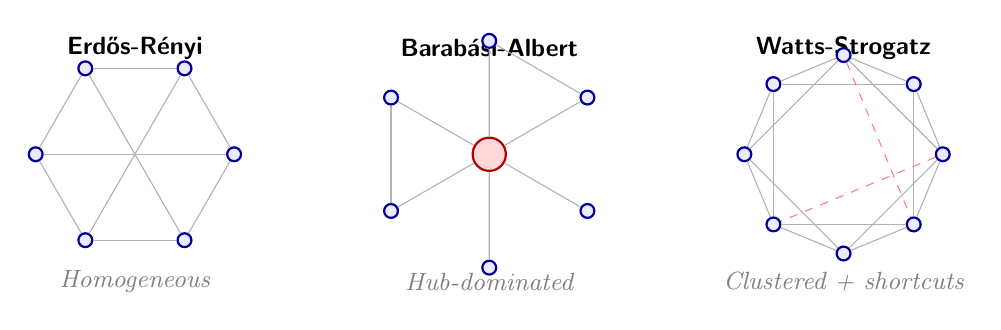
\begin{tikzpicture}[
  snode/.style={circle, draw=blue!60!black, fill=blue!8, minimum size=5pt, inner sep=0, thick},
  hnode/.style={circle, draw=red!70!black, fill=red!15, minimum size=8pt, inner sep=0, thick},
  scale=0.9
]
\node[font=\bfseries\sffamily\small] at (2.0, 3.0) {Erd\H{o}s-R\'{e}nyi};
\foreach \a in {0,...,5}{
  \node[snode] (er\a) at ({2.0+1.4*cos(60*\a)}, {1.5+1.4*sin(60*\a)}) {};
}
\foreach \a/\b in {0/1,1/2,2/3,3/4,4/5,5/0,0/3,1/4,2/5}{
  \draw[gray!60, thin] (er\a)--(er\b);
}
\node[font=\bfseries\sffamily\small] at (7.0, 3.0) {Barab\'{a}si-Albert};
\node[hnode, minimum size=12pt] (ba0) at (7.0, 1.5) {};
\foreach \i in {1,...,6}{
  \node[snode] (ba\i) at ({7.0+1.6*cos(60*\i-30)}, {1.5+1.6*sin(60*\i-30)}) {};
  \draw[gray!60, thin] (ba0)--(ba\i);
}
\draw[gray!60,thin] (ba1)--(ba2); \draw[gray!60,thin] (ba3)--(ba4);
\node[font=\bfseries\sffamily\small] at (12.0, 3.0) {Watts-Strogatz};
\foreach \i in {0,...,7}{
  \node[snode] (ws\i) at ({12.0+1.4*cos(45*\i)}, {1.5+1.4*sin(45*\i)}) {};
}
\foreach \i/\j in {0/1,1/2,2/3,3/4,4/5,5/6,6/7,7/0,0/2,1/3,2/4,3/5,4/6,5/7,6/0,7/1}{
  \draw[gray!60, thin] (ws\i)--(ws\j);
}
\draw[red!50, dashed, thin] (ws0)--(ws5);
\draw[red!50, dashed, thin] (ws2)--(ws7);
\node[font=\small\itshape, text=gray] at (2.0, -0.3) {Homogeneous};
\node[font=\small\itshape, text=gray] at (7.0, -0.3) {Hub-dominated};
\node[font=\small\itshape, text=gray] at (12.0, -0.3) {Clustered + shortcuts};
\end{tikzpicture}
\end{center}

The large red node in the BA diagram is the hub. The dashed red lines in the WS diagram are the rewired ``shortcut'' edges.

\begin{table}[H]
\centering
\caption{Comparison of standard network generation models.}
\label{tab:network_models}
\begin{tabular}{lllll}
\toprule
\textbf{Model} & \textbf{Degree dist.} & \textbf{Clustering} & \textbf{Diameter} & \textbf{Epidemic relevance} \\
\midrule
Erd\H{o}s-R\'{e}nyi & Poisson & Low $\sim K/n$ & $O(\ln n)$ & Mean-field baseline \\
Barab\'{a}si-Albert  & Power-law $k^{-3}$ & Moderate & $O(\ln n/\ln\ln n)$ & Super-spreader networks \\
Watts-Strogatz       & Peaked & High & $O(\ln n)$ & Real social/contact nets \\
Configuration        & Arbitrary & Depends & Depends & Null model \\
\bottomrule
\end{tabular}
\end{table}

% =============================================================================
\section{Comprehensive Worked Example: Building and Analysing $G_6$}
\label{sec:worked_example}
% =============================================================================

\begin{examplebox}{Step 1 --- Define the Graph}
$n=6$, $m=8$, density $\rho = 16/30 \approx 0.533$.
\end{examplebox}

\begin{examplebox}{Step 2 --- Adjacency and Degree Matrices}
\[
\mathbf{A} = \begin{pmatrix}
0&1&1&0&0&0\\1&0&1&1&0&0\\1&1&0&0&1&0\\0&1&0&0&1&1\\0&0&1&1&0&1\\0&0&0&1&1&0
\end{pmatrix}, \qquad
\mathbf{D} = \mathrm{diag}(2,3,3,3,3,2)
\]
$\mathrm{trace}(\mathbf{D}) = 16 = 2m$ \checkmark
\end{examplebox}

\begin{examplebox}{Step 3 --- Graph Laplacian}
$\mathbf{L} = \mathbf{D} - \mathbf{A}$:
\[
\mathbf{L} = \begin{pmatrix}
 2&-1&-1& 0& 0& 0\\
-1& 3&-1&-1& 0& 0\\
-1&-1& 3& 0&-1& 0\\
 0&-1& 0& 3&-1&-1\\
 0& 0&-1&-1& 3&-1\\
 0& 0& 0&-1&-1& 2
\end{pmatrix}
\]
Each row sums to zero \checkmark. Symmetric \checkmark. Diagonal entries equal degrees \checkmark.
\end{examplebox}

\begin{examplebox}{Step 4 --- $\mathbf{D}^{-1/2}$ and the Normalised Laplacian}
\[
\mathbf{D}^{-1/2} \approx \mathrm{diag}(0.707,\, 0.577,\, 0.577,\, 0.577,\, 0.577,\, 0.707)
\]
Off-diagonal entries: edges connecting degree-2 to degree-3 nodes give $-1/\sqrt{6} \approx -0.408$; degree-3 to degree-3 edges give $-1/3 \approx -0.333$. All eigenvalues in $[0,2]$.
\end{examplebox}

\begin{examplebox}{Steps 5--6 --- Metrics Summary}
\begin{center}
\begin{tabular}{ccccc}
\toprule
Node & Degree & $C_v$ & Closeness $C_C$ & Betweenness \\
\midrule
1 & 2 & 1.00 & 0.56 & 0 \\
2 & 3 & 0.33 & 0.71 & non-zero \\
3 & 3 & 0.33 & 0.71 & non-zero \\
4 & 3 & 0.33 & 0.71 & non-zero \\
5 & 3 & 0.33 & 0.71 & non-zero \\
6 & 2 & 1.00 & 0.56 & 0 \\
\bottomrule
\end{tabular}
\end{center}
$\bar{C} \approx 0.556$. Mean degree $\langle k \rangle \approx 2.67$.
\end{examplebox}

\begin{keyinsight}{Why These Matrices Matter for GNNs}
Every GNN layer performs a variant of:
\[
\mathbf{H}^{(l+1)} = \sigma\!\left(\hat{\mathbf{A}}\,\mathbf{H}^{(l)}\,\mathbf{W}^{(l)}\right)
\]
where:
\begin{itemize}[noitemsep]
    \item $\mathbf{H}^{(l)} \in \mathbb{R}^{n \times d_l}$: feature matrix at layer $l$ (one row per node)
    \item $\hat{\mathbf{A}}$: normalised adjacency (e.g.\ $\mathbf{D}^{-1/2}\mathbf{A}\mathbf{D}^{-1/2}$); multiplying by $\hat{\mathbf{A}}$ aggregates neighbours' features
    \item $\mathbf{W}^{(l)} \in \mathbb{R}^{d_l \times d_{l+1}}$: learnable weight matrix
    \item $\sigma$: non-linear activation (e.g.\ ReLU: $\sigma(x) = \max(0,x)$)
\end{itemize}

What changes between GCN, GraphSAGE, GAT, and ChebNet is \emph{precisely} which matrix plays the role of $\hat{\mathbf{A}}$. Understanding the Laplacian and its spectral properties is not abstract mathematics: it directly determines what structural information flows through each layer of every model in \texttt{gnn/}.
\end{keyinsight}

% =============================================================================
\section{Chapter Summary}
% =============================================================================

\begin{conceptbox}{What We Have Established}
\begin{enumerate}[noitemsep]
    \item \textbf{Graphs} $G = (\mathcal{V}, \mathcal{E})$ encode contact networks. The degree $k_i$ counts a node's neighbours. The handshaking lemma: $\sum_i k_i = 2m$.
    \item \textbf{Matrices:} $\mathbf{A}$ ($A_{ij}=1$ if edge exists), $\mathbf{D}$ (diagonal matrix of degrees), $\mathbf{L} = \mathbf{D}-\mathbf{A}$ (Laplacian). Every row of $\mathbf{L}$ sums to zero.
    \item \textbf{$\mathbf{D}^{-1/2}$:} For a diagonal matrix, raise each diagonal entry to the power $-1/2$ (i.e., take $1/\sqrt{d_i}$). The normalised Laplacian $\tilde{\mathbf{L}}_{\mathrm{sym}} = \mathbf{D}^{-1/2}\mathbf{L}\mathbf{D}^{-1/2}$ has eigenvalues in $[0,2]$. For $G_6$: off-diagonal entries are $-0.408$ (for 2-3 degree edges) or $-0.333$ (for 3-3 degree edges).
    \item \textbf{Eigenvectors/eigenvalues:} $\mathbf{L}\mathbf{u} = \lambda\mathbf{u}$. Smallest eigenvalue $\lambda_1 = 0$ (all-ones vector). Fiedler value $\lambda_2 > 0$ iff connected.
    \item \textbf{GFT:} $\hat{\mathbf{f}} = \mathbf{U}^\top\mathbf{f}$ decomposes a graph signal into frequency components. Graph convolution is spectral filtering. Chebyshev polynomials ($T_0=1, T_1=x, T_k=2xT_{k-1}-T_{k-2}$) make this $O(K \cdot m)$ instead of $O(n^3)$.
    \item \textbf{Network metrics:} Degree distribution, clustering, betweenness/closeness centrality, PageRank characterise local and global structure. They serve as node features in GNN models.
    \item \textbf{Generation models:} ER (homogeneous), BA (hub-dominated, $P(k)\sim k^{-3}$), WS (small-world), Configuration (arbitrary degree sequence).
\end{enumerate}
\textbf{Coming up:} Chapter~2 lifts these static definitions into the temporal domain, introducing time-stamped contact sequences, time-respecting paths, and the causal structure that makes temporal GNNs both necessary and powerful.
\end{conceptbox}
